% \section{Preliminary Work and Motivation: Real-World Bug Study}
% \label{sec:preliminary}

% Over the past two years, using a corpus of 510 bugs from real-world programs (TensorFlow~\cite{tensorlow}, MySQL~\cite{mysql}, SQLite~\cite{sqlite}, MariaDB~\cite{mariadb}, Chromium~\cite{chromium}, memcached~\cite{memcached}, Apache httpd~\cite{httpd}, nginx~\cite{nginx}, etc.), we investigated the limitations of existing bug reproduction systems. This corpus will form the foundation of our experimental evaluation~(\ref{sec:evaluation}). The largest study of real-world software bugs that we know of is from Yuan et al.~\cite{osdi12-errlog} (250 bugs). The largest \textit{reproducible} bug databases for real-world systems are from Yu et al.~\cite{jieyucon28:database} and Lin et al.~\cite{lin:jacontebe}, both of which contain an order of magnitude fewer reproducible bugs than what we included in our study (24 and 47 respectively, 71 bugs in total). We and others have used these 71 bugs in prior work~\cite{arulraj:lbr,snorlax,gist,portend,racemob,pres} and also included them in our preliminary analysis. However, several bugs in these databases date as far back as 15 years, and since our goal is to also represent bugs in modern systems, we used 439 additional recent bugs, many of which are security vulnerabilities. To ensure that these are complex bugs, we verified that none of them were found using fuzzers or automated tools.

% \begin{table}[hbt!]
%   \caption{Real-world bug study results. L stands for Latent bugs and NL stands for Non-latent bugs}
%   \label{table:study}
%   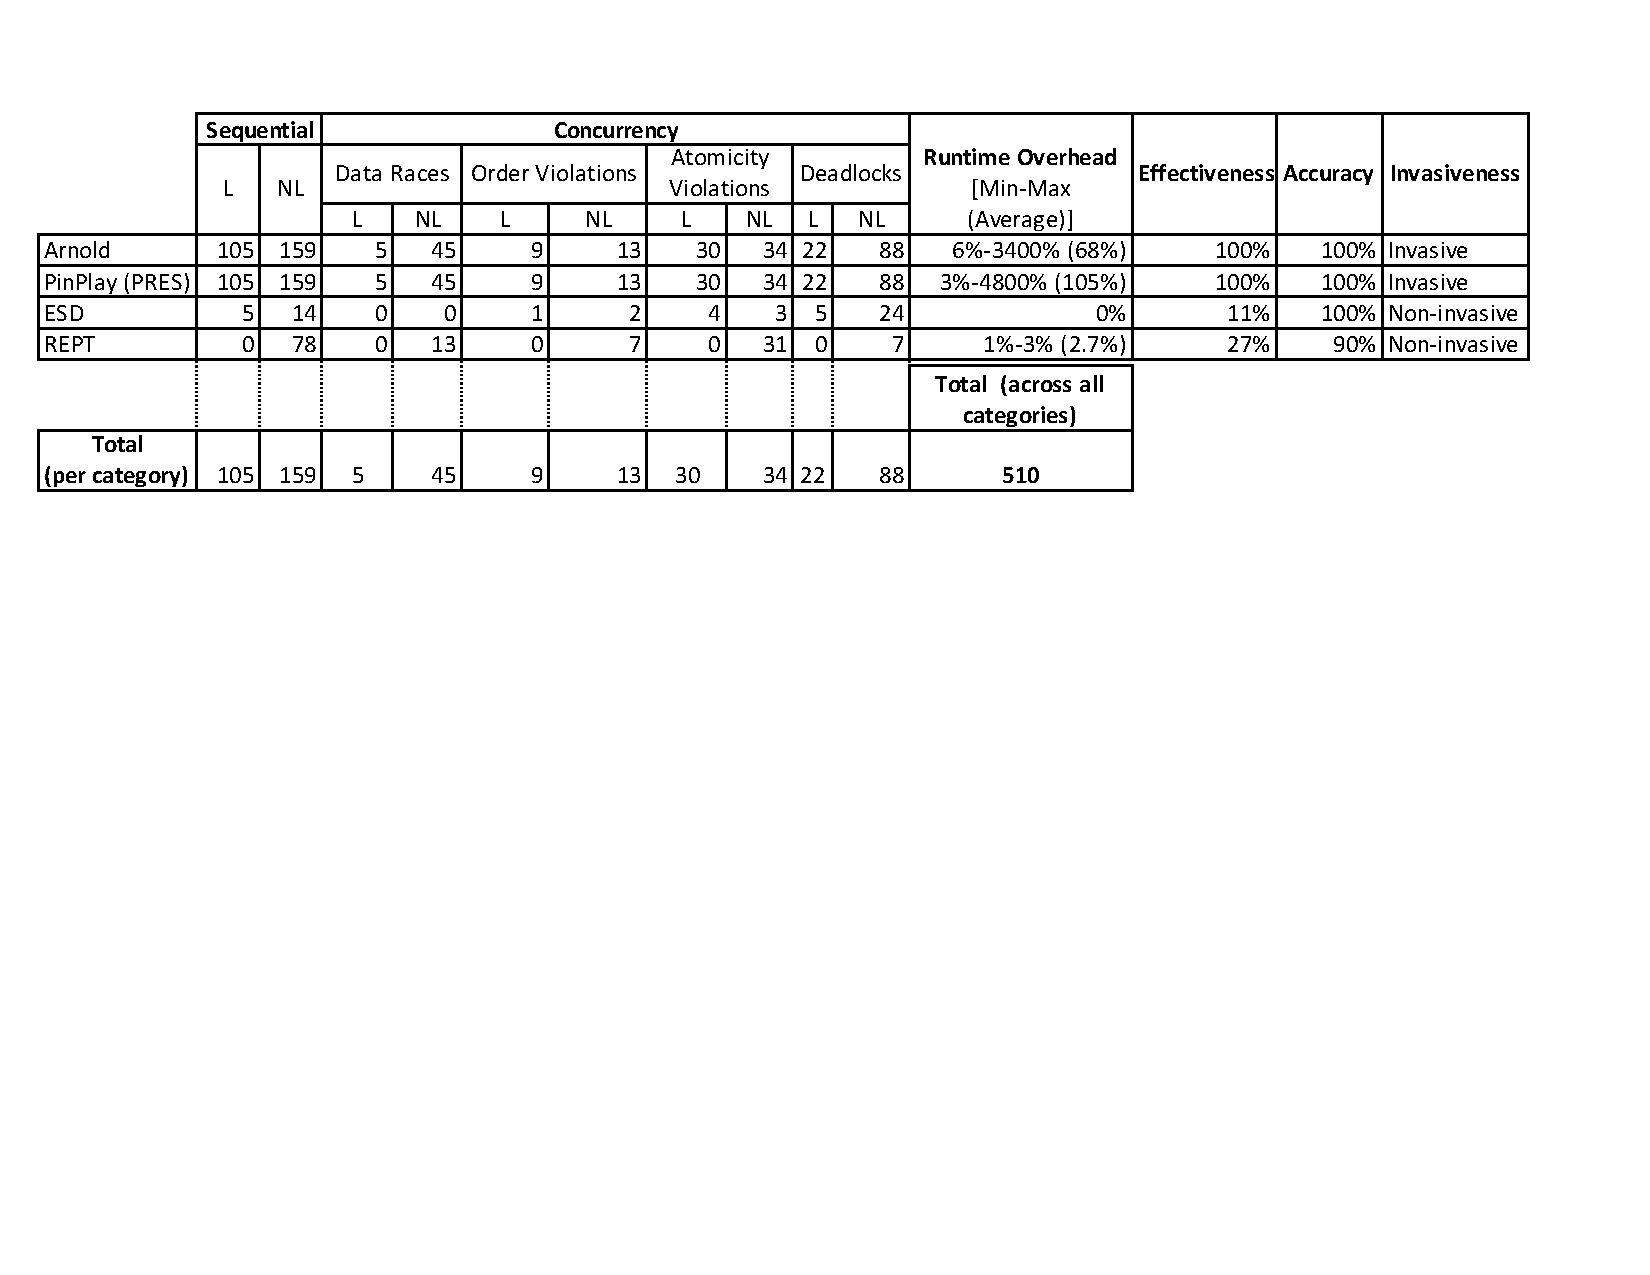
\includegraphics[width=\linewidth]{Figures/study.pdf}
% \end{table}

% Table~\ref{table:study} shows the breakdown of the bugs in our study. We wanted to equally represent concurrency bugs and sequential bugs (246 and 264 bugs, respectively), where bugs within a category are randomly selected from bug trackers. \textit{Data races}~\cite{eraser} occur when two memory accesses from different threads (at least one write) occur without an intervening happens-before relationship~\cite{lamporthb}; \textit{Order violations} occur when the order of accesses to shared data causes a failure~\cite{cfix}; \textit{Atomicity violations}~\cite{avio,atomaid,colorsafe} occur when programmers fail to enclose memory accesses that should happen atomically inside the same critical section; \textit{Deadlocks} occur when a group of processes cannot make forward progress because each process is waiting for another to release some shared resource~\cite{distrsysbook} (mainly locks). We define a latent bug as a bug with a long root-cause-to-failure distance. We define this distance as 100,000 executed instructions. We chose this threshold, because the-state-of-the-art production bug-reproduction system, REPT, can accurately reproduce buggy executions shorter than 100,000 instructions, and is ineffective for longer executions~\cite{rept}.

% We corroborate prior work that found (1) atomicity violations to be the most common non-deadlock concurrency bug (26\%)~\cite{Lu08}, and (2) most concurrency bugs to be non-latent~\cite{conseq}. The ratio of latent bugs in our study is higher than in prior work (27\% vs. 15\%). However, prior work defines a bug as latent if there are fewer than 4 control/data dependencies between the root cause and the failure. We verified that our 100,000 instruction criterion contains up to 11 control/data dependencies in that interval, making 27\% conservative. A larger percentage of sequential bugs (40\%) are latent compared to concurrency bugs~(18\%). We corroborate work drawing attention to the proliferation of latent bugs~\cite{pedrolatent,tancreti2011aveksha,tancreti2015tardis,tancreti2015phdthesis,guan2012mitigating,cinque2012analyzing}.

% We evaluated the limitations of state-of-the-art bug reproduction techniques using four systems:

% \begin{enumerate}[leftmargin=*]

% \item Arnold~\cite{arnold}: is a state-of-the-art record replay system. We chose Arnold over iReplayer~\cite{ireplayer} and Castor~\cite{castor} since the latter two systems are not available. Arnold may not handle executions with a data race, but iReplayer can, but we conservatively assume that both can reproduce all the bugs in our corpus.  

% \item PinPlay~\cite{pinplay}: is a record/replay system that uses Intel PIN~\cite{intelpin} like PRES~\cite{pres}. PRES~\cite{pres} is not available, so we assume that it can reproduce all the bugs in our corpus and evaluate PinPlay's overhead.

% \item ESD~\cite{esd}: is the execution synthesis tool~\cite{esd} that I used and extended in prior work~\cite{portend}.

% \item REPT~\cite{rept}: We implemented REPT~\cite{rept} in Linux to represent the only real-world production bug reproduction system. H3~\cite{h3} is not available, however, REPT and H3 use the same control flow tracing technology (Intel PT~\cite{intelpt}), so we think that REPT's overhead is representative of H3's overhead.

% \end{enumerate}

% \begin{wrapfigure}{R}{0.35\textwidth}
% \centering
% 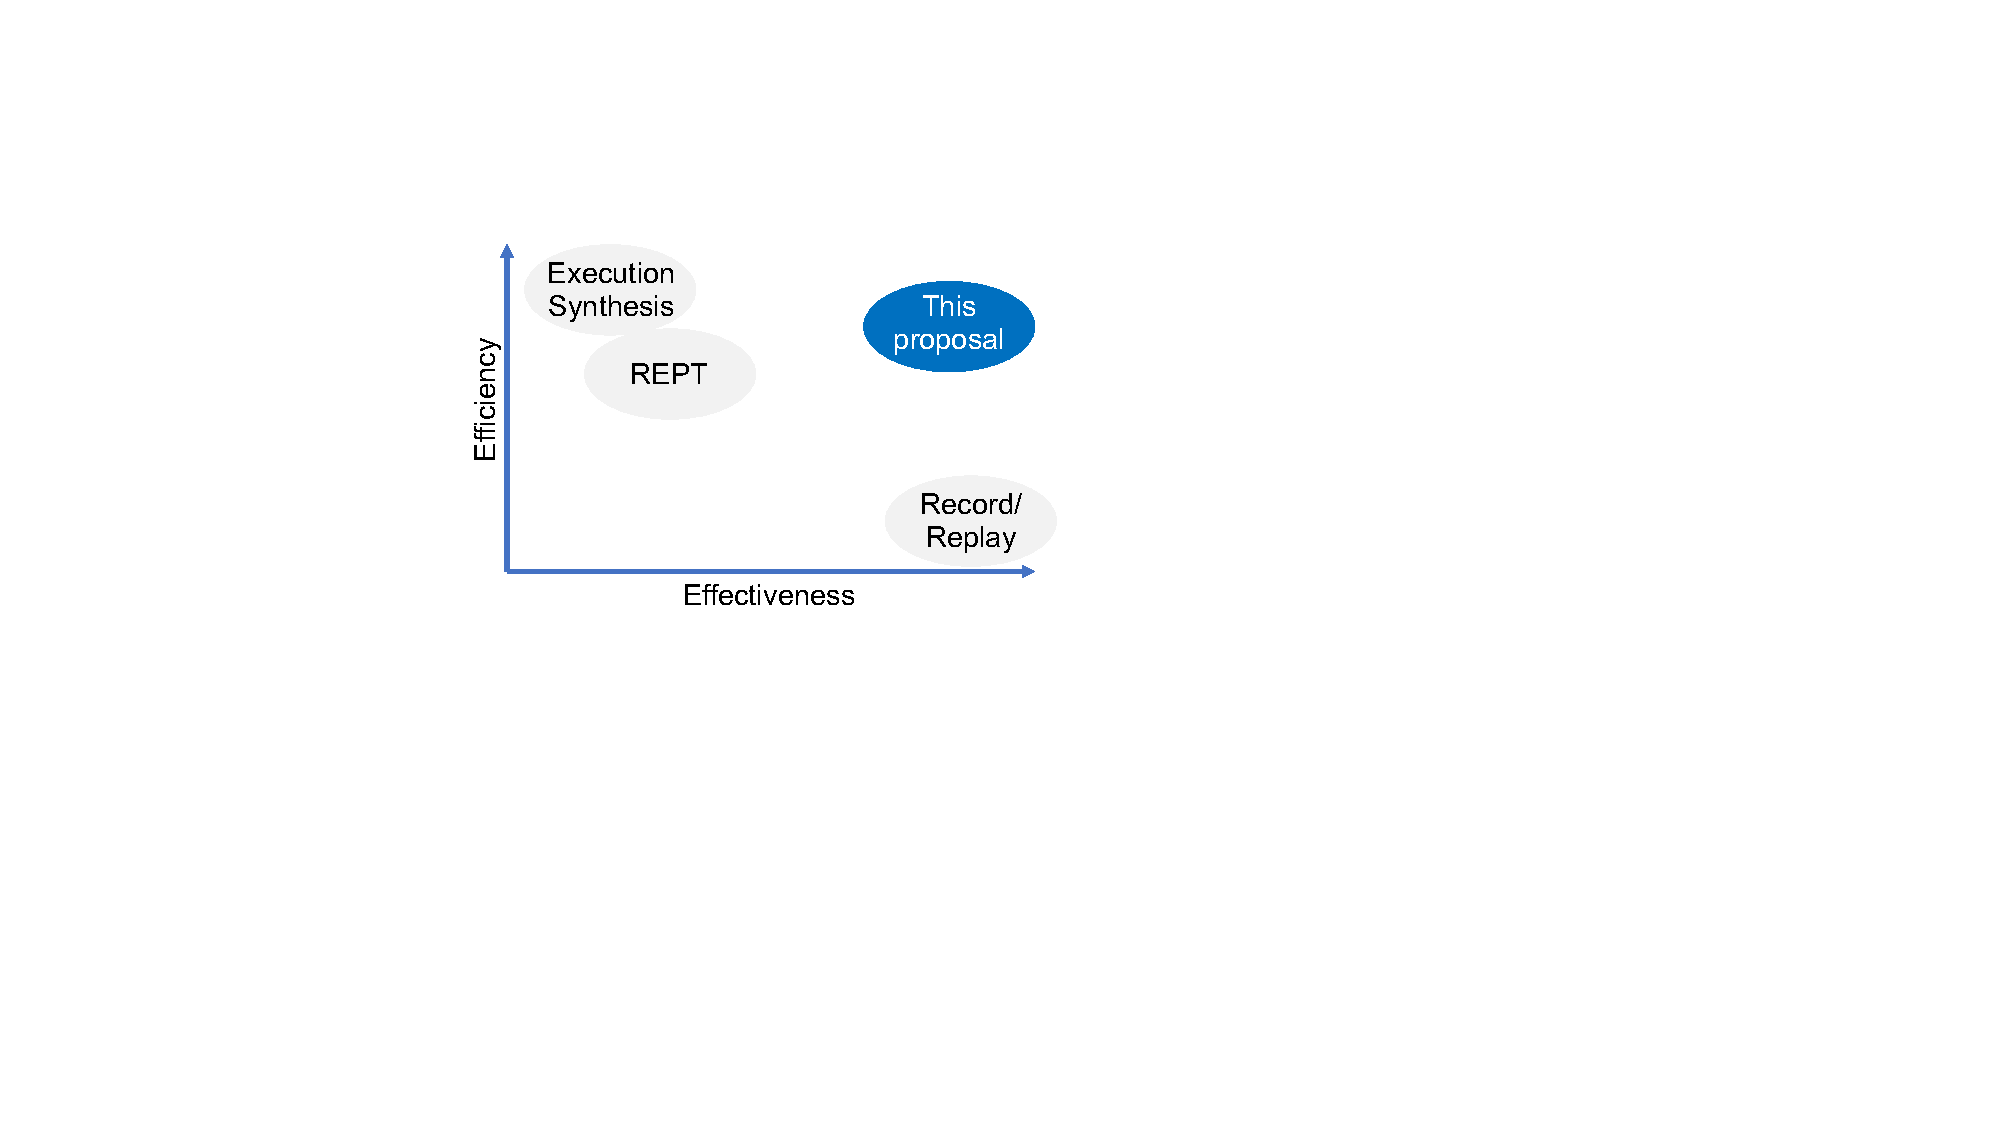
\includegraphics[width=\linewidth]{Figures/space.pdf}
% \caption{Efficiency-Effectiveness trade-off space for bug reproduction}
% \label{fig:space}
% \end{wrapfigure}


% \noindent \textbf{Summary and interpretation of results:}

% \textbf{\textit{Record/replay is expensive.}} Record/replay systems can reproduce all the bugs in our study, but may incur high overheads (34$\times$--48$\times$) for I/O intensive applications (e.g., Chromium, MySQL, etc.), making them unsuitable in production. 

% \textbf{\textit{Execution synthesis is ineffective.}} Static analysis and symbolic execution without any runtime monitoring can only reproduce a small percentage of bugs (11\%).

% \textbf{\textit{REPT is efficient but ineffective.}} REPT incurs low overhead but reproduces only 27\% of the bugs in our study and is ineffective for the rest. REPT is completely ineffective for latent bugs and less effective for concurrency bugs (23\%) than sequential bugs (30\%).

% \textbf{\textit{Existing techniques that are effective and accurate are also invasive.}} Arnold requires a custom OS, and PinPlay requires linking binaries with custom libraries and heavyweight runtime support.

% Fig.~\ref{fig:space} represents the effectiveness-efficiency trade-off, where record/replay, execution synthesis, REPT, and the techniques we propose are represented. We consider non-invasiveness and high accuracy as necessary properties of any production system. There is a tension between efficiency and effectiveness. Building effective and efficient bug reproduction systems, while preserving accuracy and non-invasiveness requires multiple scientific innovations, which we will undertake in this research.

